\documentclass[10pt,a4paper]{article}

\usepackage[utf8]{inputenc}
\usepackage[T1]{fontenc}
\usepackage[italian]{babel}
\usepackage[
  top=2.2cm,
  bottom=2.2cm,
  left=2.35cm,
  right=2.35cm
]{geometry}
\usepackage{graphicx}
\usepackage{booktabs}
\usepackage{tabularx}
\usepackage{array}
\usepackage{float}
\usepackage{enumitem}
\usepackage{amsmath}
\usepackage[hidelinks]{hyperref}
\usepackage{microtype}
\usepackage{caption}

\setlength{\parindent}{0pt}
\setlength{\parskip}{0.45em}
\setlist[itemize]{leftmargin=*,itemsep=0.15em,topsep=0.2em}
\setlist[enumerate]{leftmargin=*,itemsep=0.15em,topsep=0.2em}
\linespread{1.04}
\captionsetup{font=small}
\microtypesetup{expansion=false}

\newcommand{\autore}{Alessio Natale Scarpa \\ Alessio Pecilli}
\newcommand{\insegnamento}{Sistemi Intelligenti per Internet}
\newcommand{\annoademico}{2025--2026}

\title{\textbf{FactCheck-Agent}\\Relazione tecnica su architettura backend e fine-tuning del classificatore NLI}
\author{\autore}
\date{Progetto d'esame di \insegnamento \\ Anno Accademico \annoademico}

\begin{document}
\maketitle

\begin{abstract}
\noindent
\textbf{FactCheck-Agent} è un sistema di verifica automatica di notizie che combina recupero di evidenze dal Web, classificazione logica del claim e generazione di una spiegazione argomentata. Il progetto integra un frontend \textit{Next.js}, un livello \textit{Backend-for-Frontend} per validazione e proxying delle richieste e un backend \textit{FastAPI} orchestrato tramite \textit{LangGraph}. Il contributo scientifico principale consiste nel fine-tuning di un classificatore \textit{Natural Language Inference} basato su \texttt{cross-encoder/nli-deberta-v3-base} sul dataset \texttt{pietrolesci/nli\_fever}, con ricerca degli iperparametri su learning rate, weight decay ed epoche.

La migliore configurazione sperimentale raggiunge sul validation set un'accuracy del $74.3\%$ e un macro-F1 del $74.1\%$, con un miglioramento marcato rispetto alla baseline non fine-tunata. Dal punto di vista ingegneristico, il backend attuale implementa una pipeline a quattro nodi: raffinamento automatico della query, retrieval tramite DuckDuckGo, classificazione NLI con checkpoint DeBERTa fine-tuned locale e generazione della motivazione tramite modello generativo remoto. In questa architettura il verdetto fattuale non è affidato all'LLM, che viene utilizzato esclusivamente per supportare la ricerca e produrre una spiegazione testuale interpretabile.
\end{abstract}

\section{Introduzione}

La verifica automatica di affermazioni testuali è un problema centrale nei sistemi intelligenti per il Web, soprattutto in scenari caratterizzati da forte eterogeneità delle fonti, rapida obsolescenza dell'informazione e alta pressione temporale nella produzione del giudizio. In questo contesto, una pipeline di \textit{fact-checking} credibile non può ridursi alla sola generazione di una risposta plausibile: deve invece recuperare evidenze pertinenti, valutarne la coerenza con il claim e restituire un output strutturato e ispezionabile.

Il progetto \textbf{FactCheck-Agent}\footnote{\url{https://github.com/Alessio-Pecilli/sii-2026}. Il repository contiene codice sorgente, notebook, artefatti sperimentali e il checkpoint fine-tuned del classificatore in \texttt{backend/fever-nli-deberta}, oltre ai file \texttt{experiment\_results.csv}, \texttt{hf\_test\_predictions.csv} e alle figure usate in questa relazione.} affronta tale esigenza con una soluzione full-stack che unisce componenti di retrieval, orchestrazione agentica e inferenza NLI. L'utente inserisce una notizia o un claim in linguaggio naturale; il sistema reperisce materiale correlato dal Web, elabora un verdetto tra \texttt{SUPPORTS}, \texttt{REFUTES} e \texttt{NOT ENOUGH INFO}, e produce una spiegazione in italiano accompagnata dal contesto recuperato.

Dal punto di vista progettuale, il lavoro ha due obiettivi distinti ma complementari. Il primo è ingegneristico: realizzare un'applicazione web modulare con contratti API tipizzati, validazione multilivello e backend facilmente estendibile. Il secondo è modellistico: addestrare un classificatore NLI specializzato sul dominio FEVER, valutandone in modo quantitativo l'impatto rispetto al modello pre-addestrato di partenza. La relazione si concentra quindi sugli aspetti realmente caratterizzanti del progetto: architettura backend, pipeline di fine-tuning e interpretazione critica dei risultati.

\section{Architettura del Sistema e Backend}

\subsection{Vista d'insieme}

L'applicazione segue un'architettura a tre livelli con pattern \textit{Backend-for-Frontend} (BFF). Il frontend, sviluppato in \textit{Next.js 16} con \textit{React 19} e \textit{TypeScript}, gestisce input utente, upload di file \texttt{.txt}, visualizzazione dello stato della pipeline e rendering del report finale. Il Route Handler \texttt{/api/verify} costituisce il livello BFF: valida il payload, normalizza la richiesta e inoltra il contenuto al backend Python. Il backend, implementato in \textit{FastAPI}, espone l'endpoint REST \texttt{POST /verify} e invoca il grafo LangGraph che esegue la verifica.

\begin{table}[t]
  \centering
  \caption{Stack tecnologico per layer applicativo}
  \label{tab:stack}
  \small
  \begin{tabularx}{\textwidth}{>{\bfseries}lX}
    \toprule
    Layer & Tecnologie e ruolo \\
    \midrule
    Frontend & Next.js 16.1.6, React 19.2.3, TypeScript, Tailwind CSS 4, lucide-react per UI e visualizzazione del report \\
    BFF & Next.js Route Handler per validazione client-facing e proxy verso backend Python \\
    Backend & FastAPI, Pydantic v2, uvicorn, endpoint \texttt{/verify}, inizializzazione modelli in fase di startup \\
    Orchestrazione & LangGraph con quattro nodi operativi: \texttt{refine\_query}, \texttt{search\_web}, \texttt{nli\_classification}, \texttt{generate\_motivation} \\
    Retrieval & \texttt{DuckDuckGoSearchRun} da \texttt{langchain-community} \\
    LLM generativo & \texttt{ChatGoogleGenerativeAI} con modello \texttt{gemma-4-31b-it}, usato per raffinamento query e motivazione \\
    Classificatore NLI & checkpoint locale fine-tuned in \texttt{backend/fever-nli-deberta}; fallback a \texttt{cross-encoder/nli-deberta-v3-large} \\
    \bottomrule
  \end{tabularx}
\end{table}

\begin{figure}[t]
  \centering
  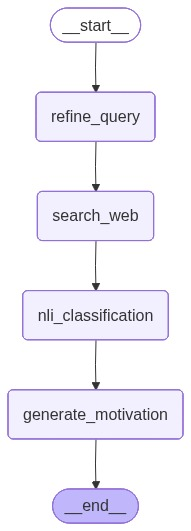
\includegraphics[width=0.27\textwidth]{figures/scheme.jpeg}
  \caption{Pipeline del backend: raffinamento query, retrieval, classificazione NLI e generazione della motivazione}
  \label{fig:scheme}
\end{figure}

La \autoref{fig:scheme} rappresenta la pipeline logica del sistema ed è coerente con l'implementazione corrente del backend. La separazione tra raffinamento della query, ricerca, classificazione logica e spiegazione finale consente di distinguere il momento decisionale supervisionato dal momento generativo esplicativo, riducendo il rischio di attribuire al modello generativo il ruolo di arbitro fattuale.

\subsection{Backend FastAPI e contratti API}

Il backend definisce schemi Pydantic fortemente tipizzati: \texttt{VerifyRequest} accetta una \texttt{query} con lunghezza compresa tra 10 e 2000 caratteri; \texttt{VerifyResponse} restituisce \texttt{verdict}, \texttt{confidence}, \texttt{explanation}, \texttt{sources}, \texttt{nli\_results}, \texttt{search\_queries} e \texttt{retrieved\_docs}. Tale struttura è replicata nel frontend tramite tipi TypeScript omologhi, riducendo il rischio di mismatch tra livelli applicativi.

L'applicazione inizializza i modelli nel \textit{lifespan} di FastAPI: il modello generativo remoto e il classificatore DeBERTa locale vengono caricati in fase di startup, mentre il grafo LangGraph viene compilato una sola volta e riutilizzato per le richieste successive. Se il workflow non è ancora disponibile, l'endpoint \texttt{POST /verify} restituisce HTTP 503.

\subsection{Grafo LangGraph e logica di esecuzione}

Nel codice attualmente deployato il grafo LangGraph è composto da quattro nodi. Il primo, \texttt{refine\_query}, utilizza il modello generativo per sintetizzare una query di ricerca breve e focalizzata. Il secondo, \texttt{search\_web}, interroga DuckDuckGo con tale query e memorizza l'output in \texttt{researches}. Il terzo, \texttt{nli\_classification}, confronta il claim utente con il testo recuperato usando il checkpoint DeBERTa fine-tuned locale, calcola i logits, applica una softmax e produce sia la classe sia la confidenza associata. Il quarto, \texttt{generate\_motivation}, costruisce una spiegazione discorsiva in italiano a partire dal verdetto NLI e dalle evidenze estratte. Il flusso è quindi:
\[
\texttt{START} \rightarrow \texttt{refine\_query} \rightarrow \texttt{search\_web} \rightarrow \texttt{nli\_classification} \rightarrow \texttt{generate\_motivation} \rightarrow \texttt{END}.
\]

Una parte ingegneristicamente rilevante è la netta separazione dei ruoli tra modelli. Il classificatore supervisionato decide il verdetto e la relativa confidenza; il modello generativo non modifica la decisione, ma contribuisce unicamente alla formulazione della query iniziale e alla spiegazione finale. Di conseguenza il campo \texttt{nli\_results} dell'API deriva da una vera inferenza del modello DeBERTa fine-tuned, mentre il testo di \texttt{explanation} rappresenta uno strato XAI discorsivo costruito sopra il risultato supervisionato.

\subsection{Ruolo del frontend e del livello BFF}

Il frontend non si limita a inviare la richiesta, ma svolge tre funzioni precise. In primo luogo, offre una validazione immediata sul claim e gestisce l'acquisizione di testo sia da textarea sia da file locali. In secondo luogo, il BFF centralizza le chiamate al backend Python e traduce errori di rete o di disponibilità in messaggi utente coerenti, ad esempio nel caso di backend non raggiungibile. In terzo luogo, il pannello risultati espone non solo il verdetto finale ma anche numero di documenti recuperati e contenuto di \texttt{nli\_results}, favorendo una forma di trasparenza operativa utile in un'applicazione di fact-checking.

Lo \textit{stepper} visuale della UI presenta i passaggi \textit{Ricerca}, \textit{NLI} e \textit{LLM} come fasi distinte. Nel backend questa separazione è effettivamente presente, anche se il primo stadio reale include un raffinamento automatico della query non esplicitato graficamente. Un limite residuo dell'implementazione corrente è invece il campo \texttt{sources}: la risposta FastAPI espone il campo per coerenza di contratto, ma l'implementazione attuale lo lascia vuoto e concentra la trasparenza sui documenti grezzi recuperati.

Un ulteriore limite metodologico riguarda la valutazione del retrieval. Nel progetto non sono state raccolte metriche quantitative come Recall@K, Precision@K o \textit{evidence hit rate} sui documenti restituiti da \texttt{DuckDuckGoSearchRun}; di conseguenza non è possibile affermare in modo misurato quante volte i documenti recuperati contengano effettivamente le evidenze necessarie per supportare o confutare il claim. L'analisi del retrieval resta quindi qualitativa: il sistema espone gli snippet recuperati, ma la loro sufficienza informativa non è stata benchmarkata contro un gold standard di evidenze.

Dal punto di vista della latenza, il repository non contiene ancora benchmark end-to-end o misure distribuzionali del tempo di risposta. È però possibile osservare che la pipeline attuale serializza due dipendenze esterne, retrieval Web e chiamata al modello generativo remoto \texttt{gemma-4-31b-it}, mentre la classificazione NLI viene eseguita localmente. Di conseguenza la latenza percepita dall'utente non dipende più dal tempo di un LLM per emettere il verdetto, ma soprattutto dal costo di rete del retrieval e della generazione della spiegazione; la decisione supervisionata resta invece, in prospettiva, il componente più prevedibile e potenzialmente più facile da ottimizzare lato serving.

\section{Processo di Fine-Tuning}

\subsection{Dataset, obiettivo e preprocessing}

Il classificatore supervisionato è addestrato nel notebook \texttt{notebooks/fever\_nli\_finetuning.ipynb} sul dataset Hugging Face \texttt{pietrolesci/nli\_fever}, che fornisce coppie \textit{premise}/\textit{hypothesis} già allineate al task di \textit{Natural Language Inference}. Le etichette utilizzate sono direttamente mappabili sul problema di fact-checking: \texttt{SUPPORTS} per entailment, \texttt{NOT ENOUGH INFO} per neutral e \texttt{REFUTES} per contradiction.

\begin{table}[t]
  \centering
  \caption{Split utilizzati nella pipeline di addestramento}
  \label{tab:splits}
  \small
  \begin{tabular}{lrrl}
    \toprule
    Split & Campioni & Label disponibili & Utilizzo \\
    \midrule
    Train & 5000 & Sì & Fine-tuning del classificatore \\
    Validation & 1000 & Sì & Selezione degli iperparametri e analisi comparativa \\
    Test & 1000 & No (\texttt{-1}) & Generazione predizioni finali in \texttt{hf\_test\_predictions.csv} \\
    \bottomrule
  \end{tabular}
\end{table}

Per contenere il costo computazionale, il notebook lavora su sottoinsiemi controllati degli split originali, riportati in \autoref{tab:splits}. La tokenizzazione è di tipo cross-encoder: premessa e ipotesi vengono fornite congiuntamente al modello con padding a lunghezza massima e troncamento a \texttt{max\_length = 256}. Questa scelta è coerente con un task di classificazione della relazione logica tra due testi, in cui l'attenzione incrociata tra le due sequenze è più importante dell'efficienza di retrieval tipica dei bi-encoder.

\subsection{Configurazione del training}

Il modello di partenza è \texttt{cross-encoder/nli-deberta-v3-base}, scelto come compromesso tra capacità rappresentativa e sostenibilità dell'addestramento su GPU T4 in ambiente Colab. La procedura di ottimizzazione esplora sei configurazioni effettive, variando \textit{learning rate}, \textit{weight decay} ed epoche. Nel training sono inoltre applicate tecniche esplicite di controllo della memoria: \textit{gradient checkpointing}, \textit{gradient accumulation} pari a 2, batch size fisico di 4 esempi e batch di valutazione di 8 esempi.

Le metriche registrate sul validation set sono accuracy, precision, recall, macro-F1 e validation loss. L'uso del macro-F1 come criterio di selezione del modello migliore è appropriato, poiché il task è tri-classe e la qualità globale del classificatore non può essere riassunta in modo affidabile dalla sola accuracy.

Gli output salvati nel notebook permettono anche di stimare il costo temporale del training su GPU T4. Le configurazioni a 2 epoche richiedono circa 8--12 minuti per run: 11:34 per \texttt{LR=1e-5, WD=0.01}, 11:51 per \texttt{LR=2e-5, WD=0.01}, 10:25 per la configurazione migliore \texttt{LR=3e-5, WD=0.1} e 08:52 per \texttt{LR=5e-5, WD=0.01}. Le configurazioni a 3 epoche completano invece il training in 13:22 (\texttt{LR=2e-5, WD=0.01}) e 14:21 (\texttt{LR=5e-6, WD=0.1}). Pur trattandosi di tempi raccolti nel contesto specifico di Colab, essi mostrano che l'intera grid search resta economicamente sostenibile su hardware didattico, mentre un retraining sistematico su dataset più ampi richiederebbe una pianificazione computazionale più rigorosa.

\section{Analisi dei Risultati e Discussione}

\subsection{Risultati della grid search}

\begin{table}[t]
  \centering
  \caption{Risultati sperimentali sul validation set da \texttt{experiment\_results.csv}}
  \label{tab:results}
  \small
  \begin{tabular}{lccccc}
    \toprule
    Modello & LR & WD & Epoche & Accuracy & Macro-F1 \\
    \midrule
    \textbf{Model\_LR\_3e-05\_WD\_0.1} & $3 \times 10^{-5}$ & 0.1 & 2 & \textbf{0.743} & \textbf{0.741} \\
    Model\_LR\_2e-05\_WD\_0.01 & $2 \times 10^{-5}$ & 0.01 & 3 & 0.737 & 0.734 \\
    Model\_LR\_2e-05\_WD\_0.01 & $2 \times 10^{-5}$ & 0.01 & 2 & 0.736 & 0.733 \\
    Model\_LR\_5e-05\_WD\_0.01 & $5 \times 10^{-5}$ & 0.01 & 2 & 0.726 & 0.722 \\
    Model\_LR\_1e-05\_WD\_0.01 & $1 \times 10^{-5}$ & 0.01 & 2 & 0.713 & 0.704 \\
    Model\_LR\_5e-06\_WD\_0.1 & $5 \times 10^{-6}$ & 0.1 & 3 & 0.645 & 0.628 \\
    \bottomrule
  \end{tabular}
\end{table}

La \autoref{tab:results} mostra una tendenza chiara. Un learning rate eccessivamente basso produce una convergenza insufficiente: la configurazione con $5 \times 10^{-6}$ si ferma a un macro-F1 di 0.628, nettamente inferiore alle altre. All'estremo opposto, il learning rate più alto testato ($5 \times 10^{-5}$) migliora la velocità di apprendimento ma non offre il miglior compromesso finale. La combinazione migliore risulta invece quella con $3 \times 10^{-5}$ e weight decay 0.1, che raggiunge il miglior equilibrio tra accuratezza e generalizzazione.

L'incremento da 2 a 3 epoche sulla configurazione con $2 \times 10^{-5}$ produce un guadagno trascurabile: accuracy da 0.736 a 0.737 e macro-F1 da 0.733 a 0.734. In termini ingegneristici, questo suggerisce che l'ottimizzazione utile si esaurisce molto rapidamente sul sottoinsieme di dati adottato e che l'aumento del tempo di training oltre le due epoche, in tale configurazione, non è giustificato da un beneficio apprezzabile.

\begin{figure}[t]
  \centering
  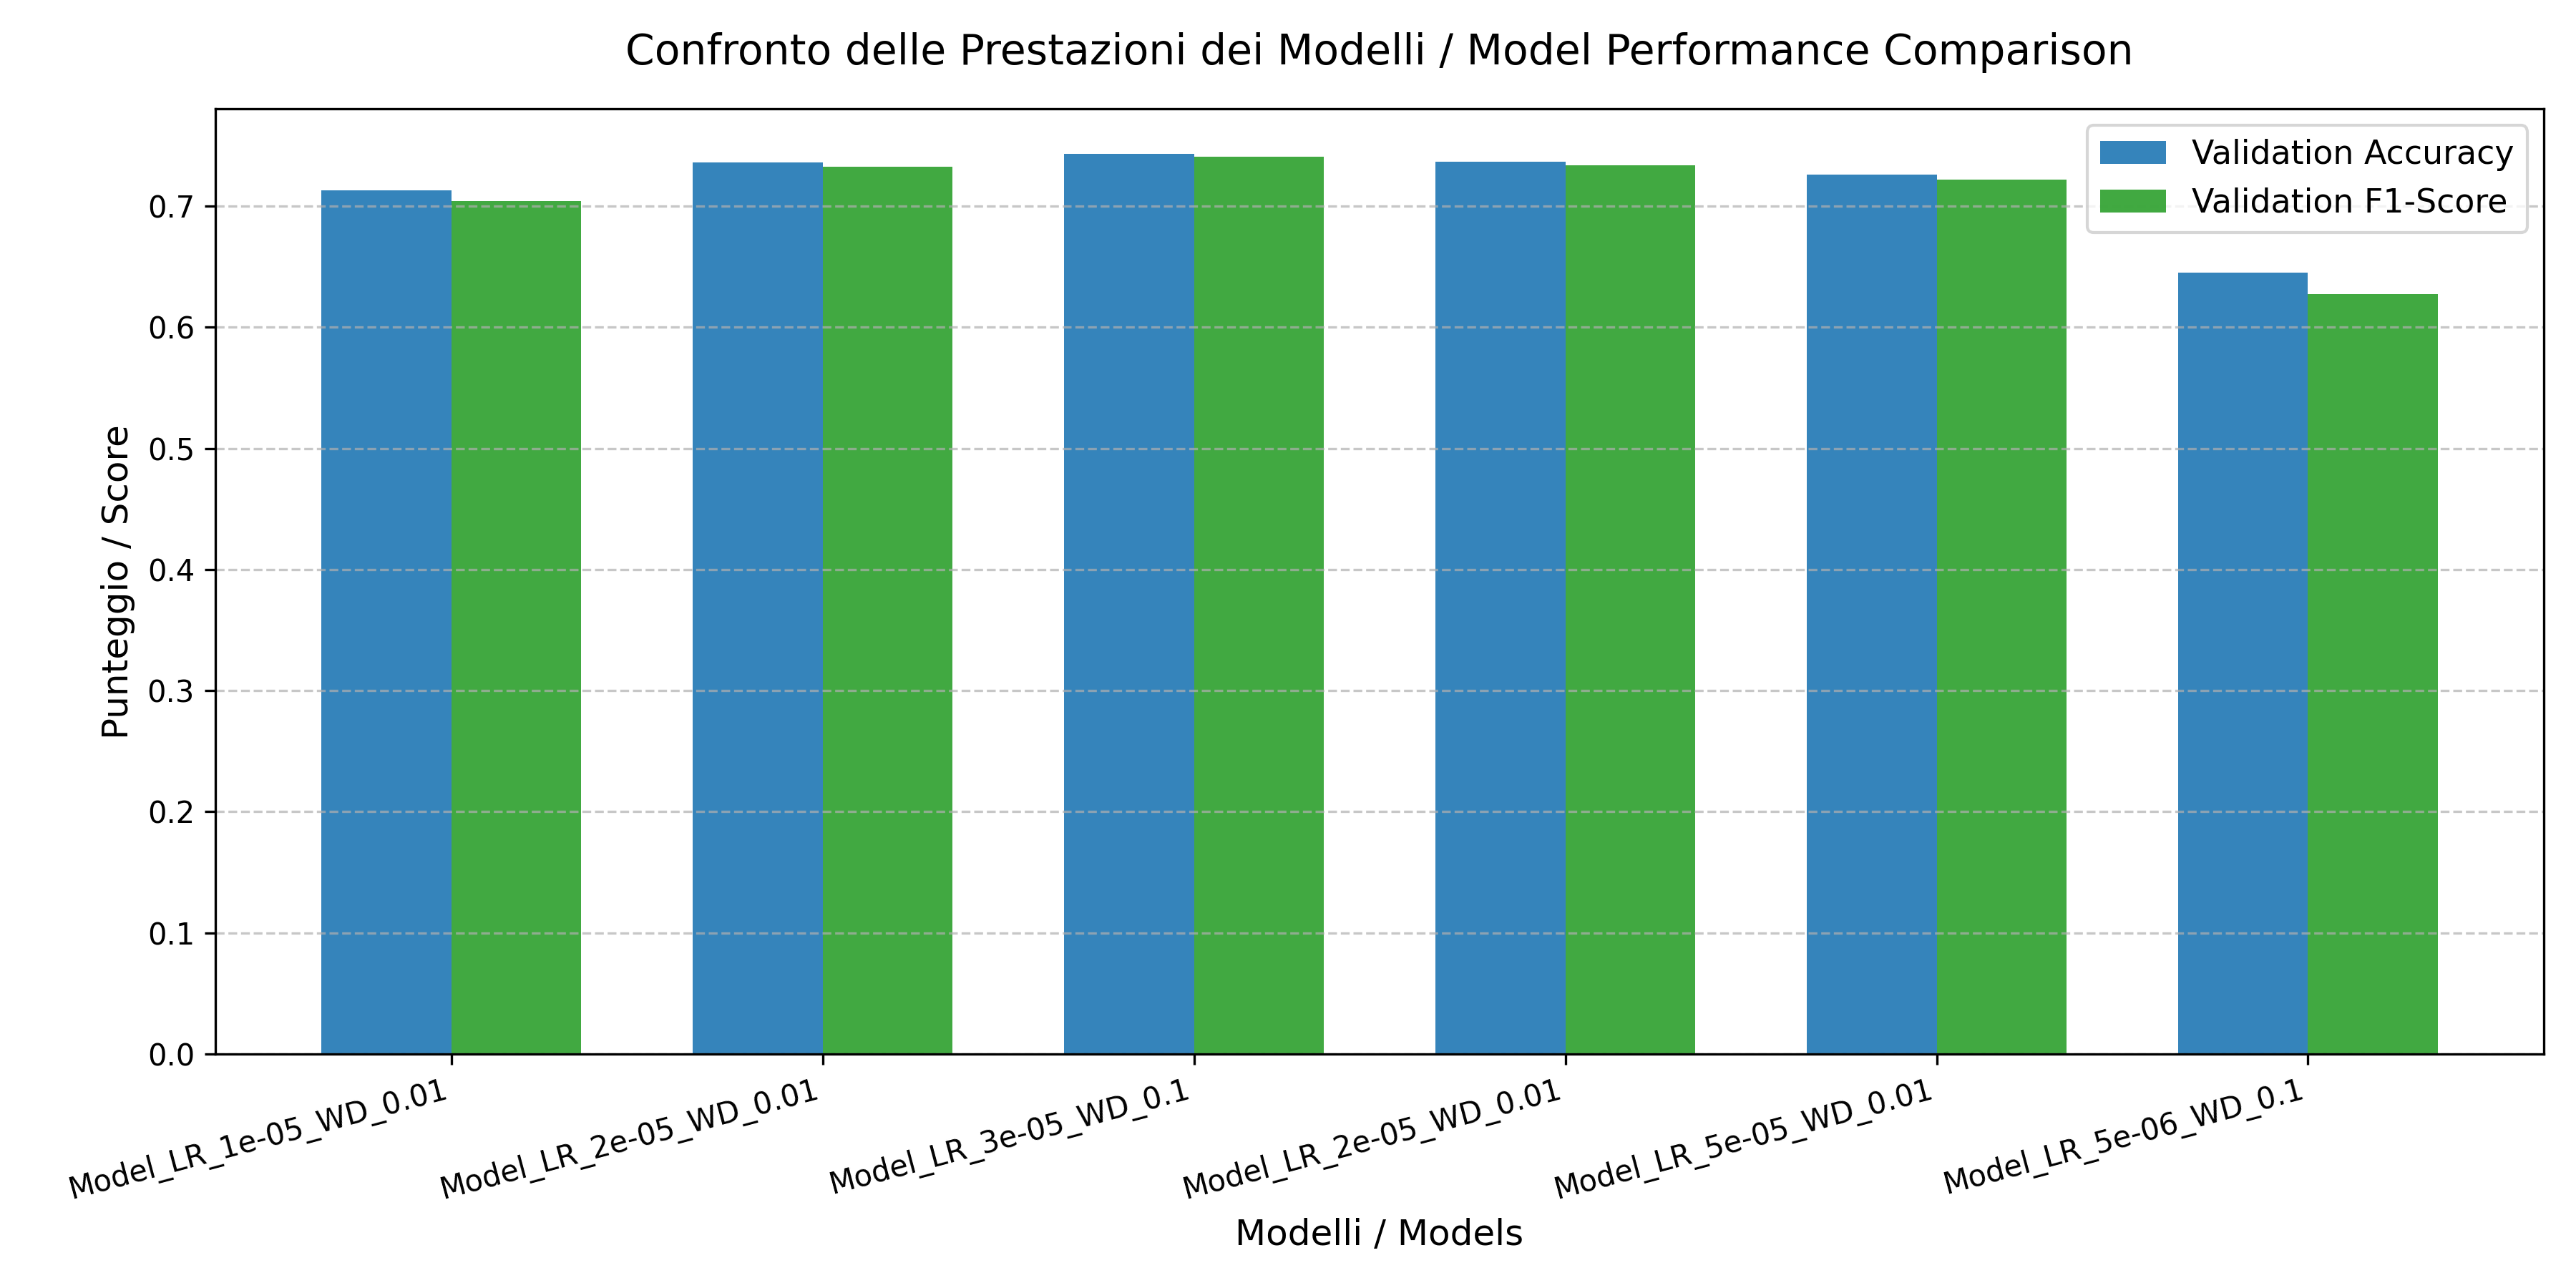
\includegraphics[width=0.83\textwidth]{figures/model_performance_comparison.png}
  \caption{Confronto tra accuracy e macro-F1 delle configurazioni esplorate}
  \label{fig:perf}
\end{figure}

\subsection{Impatto del fine-tuning}

\begin{table}[t]
  \centering
  \caption{Confronto tra baseline pre-addestrata e miglior modello fine-tuned sul validation set}
  \label{tab:baseline}
  \small
  \begin{tabular}{lcccc}
    \toprule
    Modello & Accuracy & Precision & Recall & Macro-F1 \\
    \midrule
    Base non fine-tunato & 0.1830 & 0.2472 & 0.1810 & 0.1493 \\
    \textbf{Miglior modello fine-tuned} & \textbf{0.7430} & \textbf{0.7500} & \textbf{0.7438} & \textbf{0.7406} \\
    \bottomrule
  \end{tabular}
\end{table}

Il dato più significativo dell'intera pipeline è il confronto riportato in \autoref{tab:baseline}. La baseline non fine-tunata, pur essendo già pre-addestrata su compiti NLI, mostra sul validation set una qualità del tutto insufficiente per il dominio specifico del progetto. Il fine-tuning aumenta l'accuracy di 56 punti percentuali assoluti e quasi quintuplica il macro-F1. In altre parole, il valore del progetto non risiede soltanto nell'integrazione applicativa, ma soprattutto nell'adattamento supervisionato del classificatore al dominio FEVER.

Questo risultato ha anche una lettura architetturale: il backend integra effettivamente il checkpoint fine-tuned nella pipeline online, rendendo la fase di decisione molto meno dipendente dal comportamento non deterministico del modello generativo e spostando l'LLM sul solo piano esplicativo.

\begin{figure}[t]
  \centering
  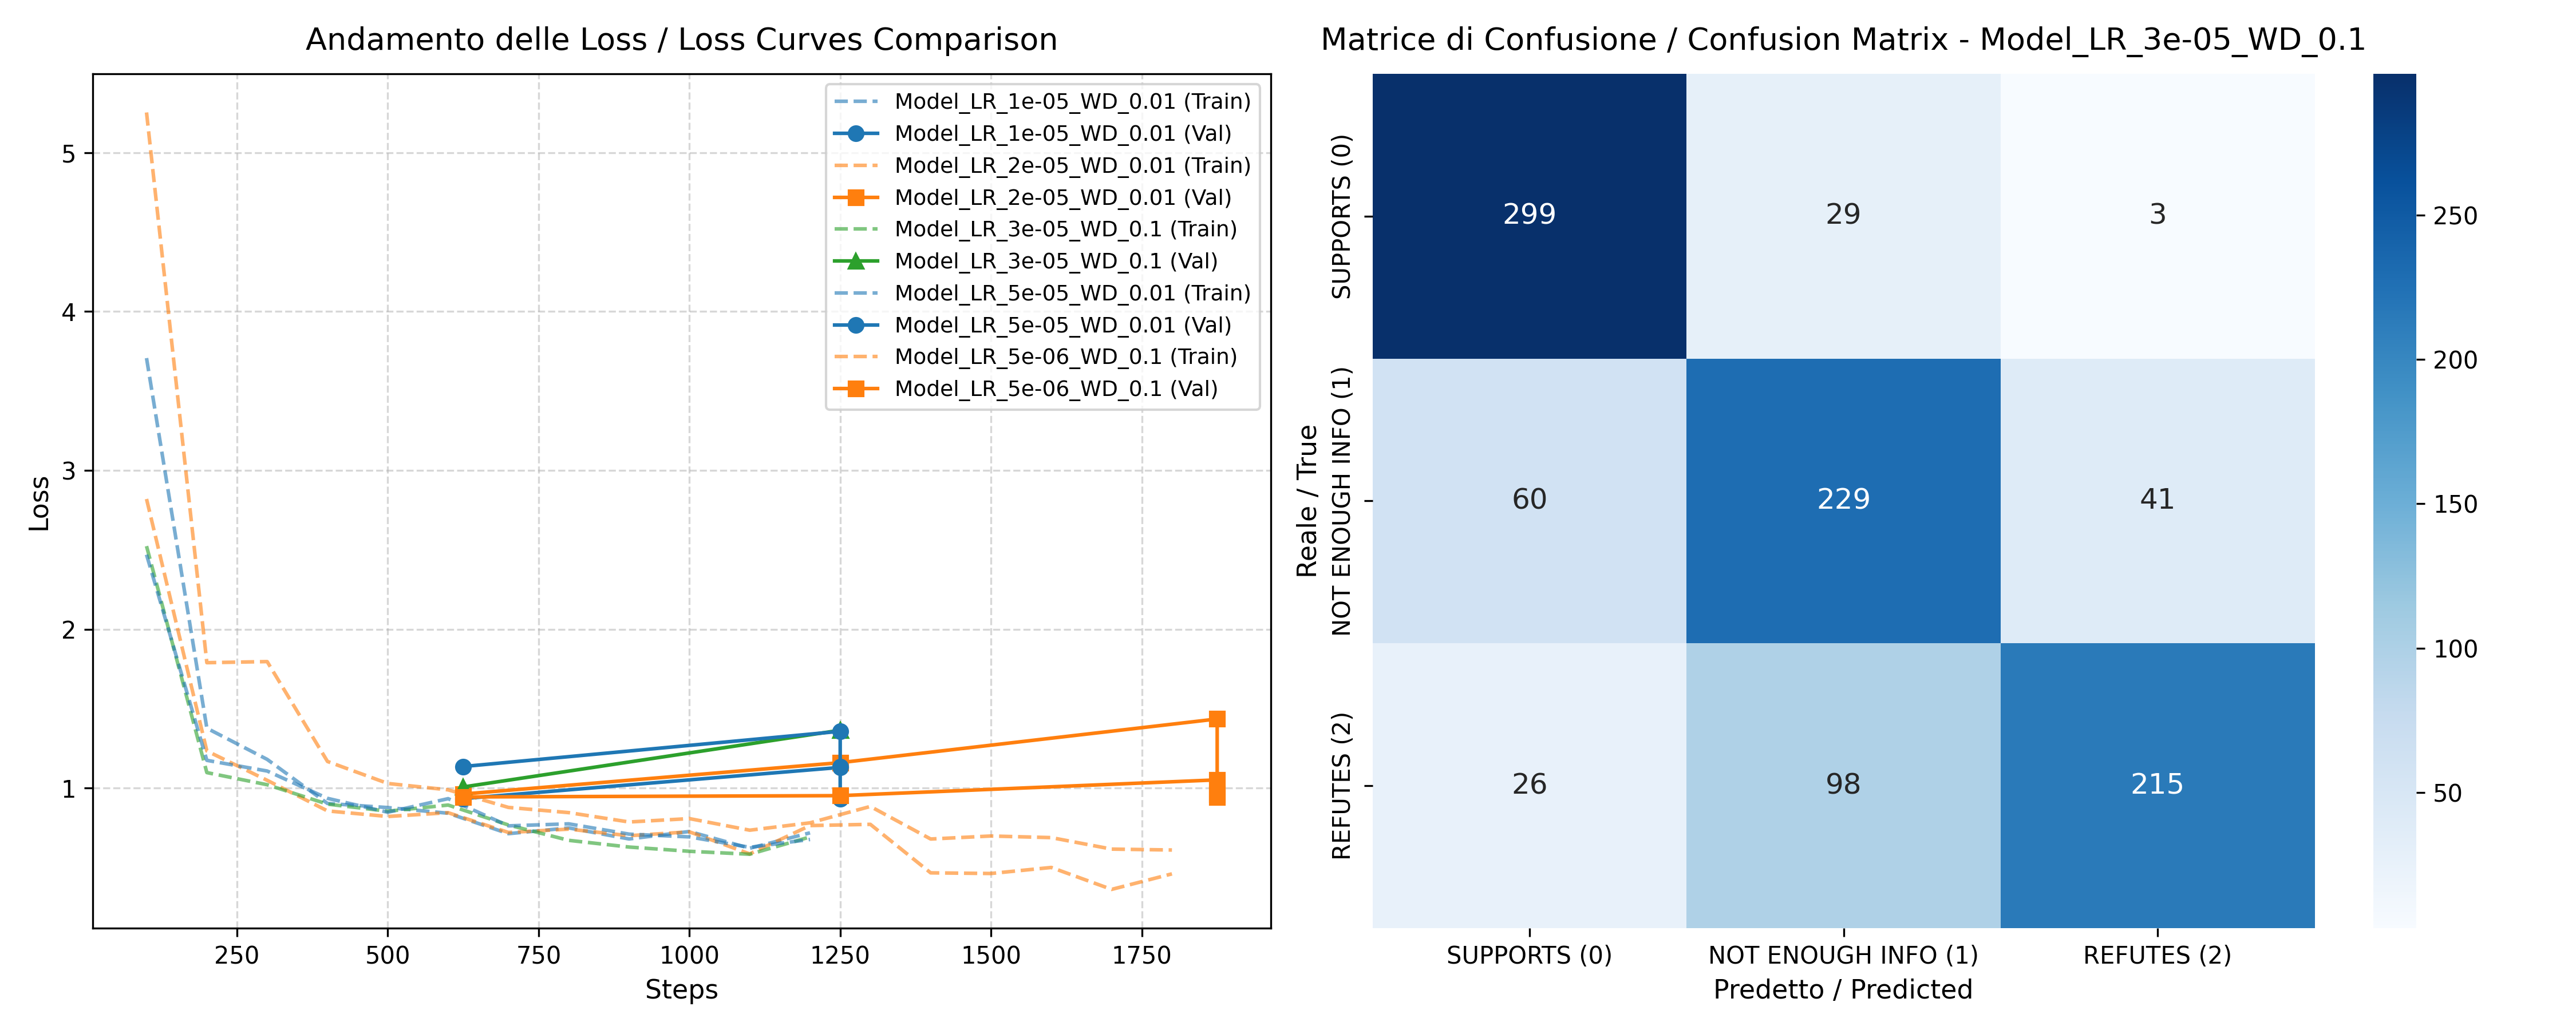
\includegraphics[width=0.84\textwidth]{figures/loss_and_confusion_matrix.png}
  \caption{Curve di loss train/validation e matrice di confusione del modello migliore}
  \label{fig:losscm}
\end{figure}

\subsection{Interpretazione qualitativa dei grafici}

Il grafico in \autoref{fig:perf} conferma visivamente la compattezza del gruppo di modelli migliori e il degrado netto delle configurazioni con learning rate troppo basso. La \autoref{fig:losscm} aggiunge due informazioni utili. In primo luogo, le curve di training e validation loss mostrano che le configurazioni migliori convergono entro poche epoche, senza evidenze marcate di overfitting sul set di sviluppo adottato. In secondo luogo, la matrice di confusione indica che la classe più problematica è \texttt{NOT ENOUGH INFO}, come atteso in un task in cui l'assenza di evidenze è semanticamente più ambigua del supporto o della contraddizione esplicita.

Va inoltre precisato che il file \texttt{hf\_test\_predictions.csv} contiene predizioni sul test split ufficiale, le cui etichette nel dataset Hugging Face sono impostate a \texttt{-1}. Di conseguenza non è possibile stimare metriche quantitative su tale insieme: il file ha valore come output di inferenza finale o come base per analisi qualitative, ma non per una validazione comparativa oggettiva.

\section{Pro, Contro e Sviluppi Futuri}

Il progetto presenta diversi punti di forza. Sul piano software, l'architettura è modulare, tipizzata e facilmente estendibile; il BFF isola il frontend dai dettagli del backend Python; il backend carica in startup sia il classificatore locale sia il modello generativo remoto e li coordina in una pipeline chiara. Sul piano modellistico, il fine-tuning è documentato, riproducibile e produce un miglioramento quantitativo molto netto rispetto alla baseline. Sul piano dell'usabilità, l'interfaccia restituisce non solo un verdetto ma anche documenti recuperati e livello di confidenza.

I limiti principali si spostano ora su altri aspetti. Il primo riguarda il retrieval: DuckDuckGo fornisce snippet testuali grezzi, utili per un prototipo ma meno controllati delle evidenze curate in FEVER, e la loro qualità non è stata misurata con metriche standard. Il secondo riguarda la spiegazione: il testo generato dal modello remoto è coerente con il verdetto supervisionato, ma resta comunque un passaggio generativo non garantito da una struttura citazionale formale. Il terzo limite è infrastrutturale: il sistema non include persistenza, rate limiting, logging strutturato o calibrazione formale della confidence. Un quarto limite applicativo è che il campo \texttt{sources} dell'API non è ancora popolato automaticamente.

Le evoluzioni più naturali sono quindi tre. La prima è il miglioramento del retrieval mediante re-ranking semantico o selezione di fonti più affidabili. La seconda è l'arricchimento dell'output con fonti esplicite e con una spiegazione più strutturata, ad esempio con citazioni ancorate alle evidenze. La terza è la trasformazione dell'architettura in un deployment più esplicito, ad esempio separando frontend, API backend e model server, così da mantenere distinto il servizio di inferenza classificatoria dal servizio generativo.

\section{Conclusione}

FactCheck-Agent dimostra che una pipeline di fact-checking ben progettata richiede sia una buona architettura software, sia un componente di inferenza specializzato e valutato in modo rigoroso. Il repository contiene entrambe le dimensioni: una web app completa, un backend agentico a quattro nodi e un percorso di fine-tuning supervisionato con risultati convincenti. La parte più forte del progetto è il classificatore NLI fine-tuned, che porta il modello da prestazioni quasi inutilizzabili a un macro-F1 di circa 0.74 sul validation set e che partecipa direttamente alla decisione online.

Dal punto di vista ingegneristico, il backend attuale rappresenta un prototipo credibile perché separa il livello decisionale supervisionato dal livello esplicativo generativo. La conclusione più importante è quindi che il progetto non si limita più a proporre l'integrazione futura tra ricerca e sistema operativo: tale integrazione è già presente nella pipeline corrente. I margini di miglioramento riguardano soprattutto la qualità del retrieval, la strutturazione delle fonti e la maturazione infrastrutturale del servizio.

\begin{thebibliography}{9}

\bibitem{thorne2018fever}
J. Thorne, A. Vlachos, C. Christodoulopoulos e A. Mittal.
\newblock FEVER: a large-scale dataset for Fact Extraction and VERification.
\newblock In \textit{Proceedings of NAACL-HLT}, 2018.

\bibitem{he2021deberta}
P. He, X. Liu, J. Gao e W. Chen.
\newblock DeBERTa: Decoding-enhanced BERT with disentangled attention.
\newblock In \textit{International Conference on Learning Representations}, 2021.

\bibitem{wolf2020transformers}
T. Wolf et al.
\newblock Transformers: State-of-the-art natural language processing.
\newblock In \textit{Proceedings of EMNLP: System Demonstrations}, 2020.

\bibitem{fastapi}
S. Ramírez.
\newblock FastAPI documentation.
\newblock \url{https://fastapi.tiangolo.com/}

\bibitem{langgraph}
LangChain Inc.
\newblock LangGraph documentation.
\newblock \url{https://langchain-ai.github.io/langgraph/}

\end{thebibliography}

\end{document}
